% Options for packages loaded elsewhere
\PassOptionsToPackage{unicode}{hyperref}
\PassOptionsToPackage{hyphens}{url}
%
\documentclass[
]{article}
\title{Esophageal Cancer}
\usepackage{etoolbox}
\makeatletter
\providecommand{\subtitle}[1]{% add subtitle to \maketitle
  \apptocmd{\@title}{\par {\large #1 \par}}{}{}
}
\makeatother
\subtitle{Esophagectomy}
\author{Jonathan Salo MD}
\date{}

\usepackage{amsmath,amssymb}
\usepackage{lmodern}
\usepackage{iftex}
\ifPDFTeX
  \usepackage[T1]{fontenc}
  \usepackage[utf8]{inputenc}
  \usepackage{textcomp} % provide euro and other symbols
\else % if luatex or xetex
  \usepackage{unicode-math}
  \defaultfontfeatures{Scale=MatchLowercase}
  \defaultfontfeatures[\rmfamily]{Ligatures=TeX,Scale=1}
\fi
% Use upquote if available, for straight quotes in verbatim environments
\IfFileExists{upquote.sty}{\usepackage{upquote}}{}
\IfFileExists{microtype.sty}{% use microtype if available
  \usepackage[]{microtype}
  \UseMicrotypeSet[protrusion]{basicmath} % disable protrusion for tt fonts
}{}
\makeatletter
\@ifundefined{KOMAClassName}{% if non-KOMA class
  \IfFileExists{parskip.sty}{%
    \usepackage{parskip}
  }{% else
    \setlength{\parindent}{0pt}
    \setlength{\parskip}{6pt plus 2pt minus 1pt}}
}{% if KOMA class
  \KOMAoptions{parskip=half}}
\makeatother
\usepackage{xcolor}
\IfFileExists{xurl.sty}{\usepackage{xurl}}{} % add URL line breaks if available
\IfFileExists{bookmark.sty}{\usepackage{bookmark}}{\usepackage{hyperref}}
\hypersetup{
  pdftitle={Esophageal Cancer},
  pdfauthor={Jonathan Salo MD},
  hidelinks,
  pdfcreator={LaTeX via pandoc}}
\urlstyle{same} % disable monospaced font for URLs
\usepackage[margin=1in]{geometry}
\usepackage{graphicx}
\makeatletter
\def\maxwidth{\ifdim\Gin@nat@width>\linewidth\linewidth\else\Gin@nat@width\fi}
\def\maxheight{\ifdim\Gin@nat@height>\textheight\textheight\else\Gin@nat@height\fi}
\makeatother
% Scale images if necessary, so that they will not overflow the page
% margins by default, and it is still possible to overwrite the defaults
% using explicit options in \includegraphics[width, height, ...]{}
\setkeys{Gin}{width=\maxwidth,height=\maxheight,keepaspectratio}
% Set default figure placement to htbp
\makeatletter
\def\fps@figure{htbp}
\makeatother
\setlength{\emergencystretch}{3em} % prevent overfull lines
\providecommand{\tightlist}{%
  \setlength{\itemsep}{0pt}\setlength{\parskip}{0pt}}
\setcounter{secnumdepth}{-\maxdimen} % remove section numbering
\usepackage{float}
\let\origfigure\figure
\let\endorigfigure\endfigure
\renewenvironment{figure}[1][2] {
    \expandafter\origfigure\expandafter[H]
} {
    \endorigfigure
}
\ifLuaTeX
  \usepackage{selnolig}  % disable illegal ligatures
\fi

\begin{document}
\maketitle

\hypertarget{introduction}{%
\section{Introduction}\label{introduction}}

I'm Dr Jonathan Salo, a GI Cancer Surgeon in Charlotte, North Carolina.

In this video, you will learn about

\begin{itemize}
\tightlist
\item
  Different kinds of surgery for esophageal cancer
\item
  Risks of surgery
\item
  How you can reduce the risk of surgery
\end{itemize}

In another video, we'll talk about how to choose a hospital and surgeon
for your esophagectomy.

\begin{center}\rule{0.5\linewidth}{0.5pt}\end{center}

Surgery for esophageal cancer is generally performed for three different
situations:

\begin{itemize}
\tightlist
\item
  Superficial Tumors (T1) that can't be completely removed by endoscopy
\item
  Localized Tumors (T2N0)
\item
  Locally Advanced Tumors (T3 or N+) after the completion of
  chemotherapy and radiation
\end{itemize}

If you haven't seen it already, this may be a good time to view the
Esophageal Cancer Treatment Options video.

\begin{center}\rule{0.5\linewidth}{0.5pt}\end{center}

\hypertarget{goals-of-esophagectomy}{%
\section{Goals of Esophagectomy}\label{goals-of-esophagectomy}}

.pull-left{[} - Remove tumor from esophagus - Remove surrounding lymph
nodes - Create a new esophagus{]}

.pull-right{[} {]}

\begin{center}\rule{0.5\linewidth}{0.5pt}\end{center}

\hypertarget{resection}{%
\section{Resection}\label{resection}}

.pull-left{[}{]}

.pull-right{[} {]}

\begin{center}\rule{0.5\linewidth}{0.5pt}\end{center}

\hypertarget{reconstruction}{%
\section{Reconstruction}\label{reconstruction}}

.pull-left{[}{]}

.pull-right{[} {]}

\begin{center}\rule{0.5\linewidth}{0.5pt}\end{center}

\hypertarget{ivor-lewis-esophagectomy}{%
\section{Ivor Lewis esophagectomy}\label{ivor-lewis-esophagectomy}}

.pull-left{[}The new esophagus is now brought up into the chest. A new
connection is made between the esophagus and the stomach, called an
\emph{anastomosis}.{]}

.pull-right{[} {]}

\begin{center}\rule{0.5\linewidth}{0.5pt}\end{center}

\hypertarget{open-esophagectomy}{%
\section{Open Esophagectomy}\label{open-esophagectomy}}

.pull-left{[}Open esophagectomy requires incisions in the abdomen and
the right chest, and is a well-established surgical approach in use for
the past 75 years.{]}

.pull-right{[}{]}

\begin{center}\rule{0.5\linewidth}{0.5pt}\end{center}

\hypertarget{minimally-invasive-ivor-lewis}{%
\section{Minimally-invasive Ivor
Lewis}\label{minimally-invasive-ivor-lewis}}

.pull-left{[}Mininally-invasive esophagectomy uses small incisions in
the abdomen and chest.{]}

.pull-right{[}{]}

\begin{center}\rule{0.5\linewidth}{0.5pt}\end{center}

\hypertarget{minimally-invasive-ivor-lewis-1}{%
\section{Minimally-invasive Ivor
Lewis}\label{minimally-invasive-ivor-lewis-1}}

.pull-left{[}We have found this is the best option for most of our
patients{]}

.pull-right{[}{]}

\begin{center}\rule{0.5\linewidth}{0.5pt}\end{center}

\hypertarget{total-esophagectomy}{%
\section{Total Esophagectomy}\label{total-esophagectomy}}

.pull-left{[}For patients with tumors in the upper esophagus, we need to
remove more of the esophagus{]}

.pull-right{[}{]}

\begin{center}\rule{0.5\linewidth}{0.5pt}\end{center}

\hypertarget{total-esophagectomy-1}{%
\section{Total Esophagectomy}\label{total-esophagectomy-1}}

.pull-left{[}For patients with tumors in the upper esophagus, we need to
remove more of the esophagus{]}

.pull-right{[}{]}

\begin{center}\rule{0.5\linewidth}{0.5pt}\end{center}

\hypertarget{minimally-invasive-mckeown-esophagectomy}{%
\section{Minimally-invasive McKeown
Esophagectomy}\label{minimally-invasive-mckeown-esophagectomy}}

.pull-left{[}In this case, a connection between the esophagus and the
stomach is made in the neck.{]}

.pull-right{[}{]}

\begin{center}\rule{0.5\linewidth}{0.5pt}\end{center}

\hypertarget{transhiatal-esophagectomy}{%
\section{Transhiatal Esophagectomy}\label{transhiatal-esophagectomy}}

.pull-left{[}Another option is a transhiatal esohagectomy, which avoids
the need to make incisions in the right chest.{]}

.pull-right{[}{]}

\begin{center}\rule{0.5\linewidth}{0.5pt}\end{center}

When you meet with your surgeon, you will have an opportunity to meet
with your surgeon to discuss your particular situation and their
recommendation for surgery.

\begin{center}\rule{0.5\linewidth}{0.5pt}\end{center}

\hypertarget{risks-of-surgery}{%
\section{Risks of Surgery}\label{risks-of-surgery}}

An esophagectomy is a substantial operation, and there can be
postoperative complications. We're going to talk about two of these
complications and how you can reduce your risk of complications:

\begin{itemize}
\tightlist
\item
  Anastomotic leak
\item
  Pneumonia
\end{itemize}

\begin{center}\rule{0.5\linewidth}{0.5pt}\end{center}

\hypertarget{anastomotic-leak}{%
\section{Anastomotic Leak}\label{anastomotic-leak}}

.pull-left{[}The anastomosis is surigcal connection between the
esophagus and the stomach. {]}

.pull-right{[}{]}

\begin{center}\rule{0.5\linewidth}{0.5pt}\end{center}

\hypertarget{anastomotic-leak-1}{%
\section{Anastomotic Leak}\label{anastomotic-leak-1}}

.pull-left{[}If anastomosis does not heal properly, this can cause a
leakage of fluid from the esophagus, called an anastomotic leak.{]}

.pull-right{[}{]}

\begin{center}\rule{0.5\linewidth}{0.5pt}\end{center}

\hypertarget{anastomotic-leak-2}{%
\section{Anastomotic Leak}\label{anastomotic-leak-2}}

In some cases, the leak will heal on its own, but other cases may
require additional procedures or even surgery. The risk of leak depends
upon the operation performed but also depends upon the experience of the
surgeon. At the end of this video we have a link to a video about how to
choose a hospital and a surgeon, which talks further about the risks of
a leak.

\begin{center}\rule{0.5\linewidth}{0.5pt}\end{center}

\hypertarget{pneumonia}{%
\section{Pneumonia}\label{pneumonia}}

.pull-left{[}Pneumonia is another complication which can occurs in about
10-15\% of patients after esophagectomy. Pneumonia requires treatment
with antibiotics and frequently requires a longer hospitalization.{]}

.pull\_right{[}{]}

\begin{center}\rule{0.5\linewidth}{0.5pt}\end{center}

\hypertarget{preventing-pneumonia}{%
\section{Preventing Pneumonia}\label{preventing-pneumonia}}

There are two important ways to help prevent pneumonia after surgery:

\begin{itemize}
\tightlist
\item
  Deep breathing
\item
  Walking
\end{itemize}

\begin{center}\rule{0.5\linewidth}{0.5pt}\end{center}

\hypertarget{deep-breathing}{%
\section{Deep breathing}\label{deep-breathing}}

After surgery, it's important to breathe deeply to help your lungs
recover after surgery. After surgery, deep breathing can be
uncomfortable, so controlling your pain will be an important part of
your recovery.

\begin{center}\rule{0.5\linewidth}{0.5pt}\end{center}

\hypertarget{walking}{%
\section{Walking}\label{walking}}

Walking after surgery is also an important way to help your lungs
recover as well. When we walk, it's easier for our lungs to function.

\hypertarget{preventing-pneumonia-1}{%
\section{Preventing Pneumonia}\label{preventing-pneumonia-1}}

How can we prevent pneumonia? Believe it or not, I can tell who is more
likely to develop pneumonia after surgery when I first meet them and
shake their hand. Someone with a firm handshake has a lower risk of
pneumonia. We think this is because someone with a firm handshake
probably has good muscle tone, and someone with good muscle tone
probably has good function of the muscles between the ribs so that they
have a nice strong cough and can prevent pneumonia.

\hypertarget{strength}{%
\section{Strength}\label{strength}}

In our clinic, we actually measure your strength with a hand-held
strength gauge called a dynamometer. Based upon these measurements, we
can identify patients who may be at risk of pneumonia.

\hypertarget{patient-health-and-esophagectomy-outcomes}{%
\section{Patient Health and Esophagectomy
Outcomes}\label{patient-health-and-esophagectomy-outcomes}}

About half of our patients have good strength, shown in green. A quarter
are have low strength, shown in red Another quarter are in the middle,
shown in yellow

\begin{center}\rule{0.5\linewidth}{0.5pt}\end{center}

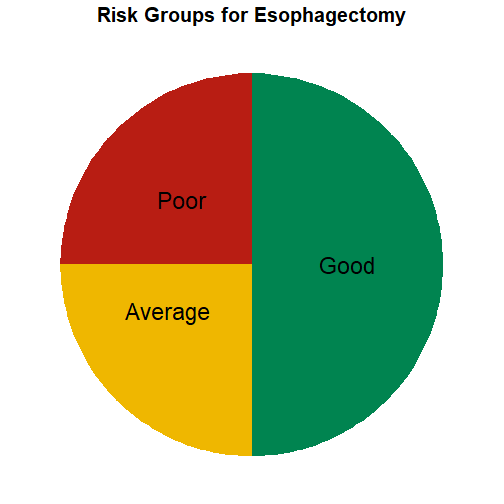
\includegraphics{12-Eso_Surgery_files/figure-latex/pie-1.pdf}

\begin{center}\rule{0.5\linewidth}{0.5pt}\end{center}

\hypertarget{pneumonia-1}{%
\section{Pneumonia}\label{pneumonia-1}}

Overall, the risk of pneumonia is about 10\% in our patients who undergo
esophagectomy. 90\% of patients never experience pneumonia, but 10\%
will have pneumonia after surgery.

\begin{center}\rule{0.5\linewidth}{0.5pt}\end{center}

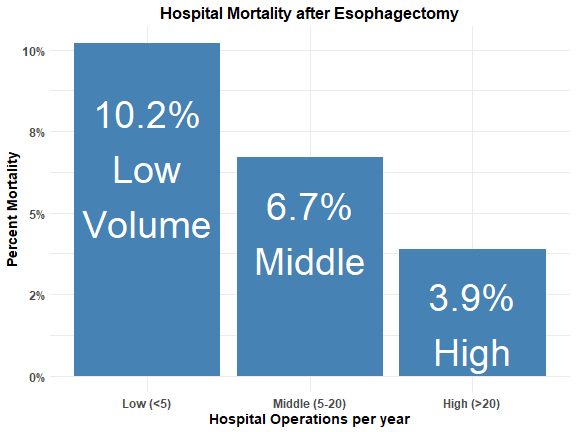
\includegraphics{12-Eso_Surgery_files/figure-latex/unnamed-chunk-1-1.pdf}

\begin{center}\rule{0.5\linewidth}{0.5pt}\end{center}

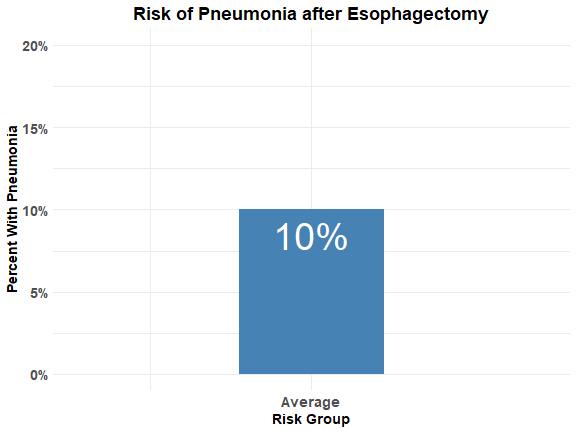
\includegraphics{12-Eso_Surgery_files/figure-latex/pneumonia_figoverall-1.pdf}

\begin{center}\rule{0.5\linewidth}{0.5pt}\end{center}

However the risk of pneumonia is not the same for everyone. Even though
the average risk is 10\%, the risk is much higher for our poor risk
patients and much lower for our good risk patients.

For the half of our patients who are in good overall health, the risk of
pneumonia is about 5\%. On the other hand, the risk of pneumonia is 20\%
in the quarter of our patients who are in poor health.

\begin{center}\rule{0.5\linewidth}{0.5pt}\end{center}

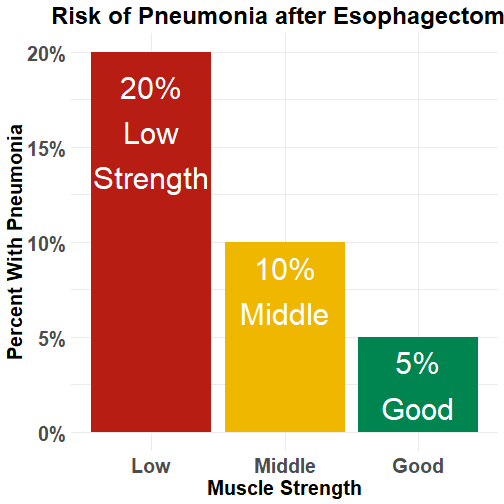
\includegraphics{12-Eso_Surgery_files/figure-latex/pneumonia_fig2b-1.pdf}

\begin{center}\rule{0.5\linewidth}{0.5pt}\end{center}

\hypertarget{muscle-strength-and-risk-after-esophagectomy}{%
\section{Muscle Strength and Risk after
Esophagectomy}\label{muscle-strength-and-risk-after-esophagectomy}}

.pull-left{[}The results of our research suggest a simple answer: The
risk of pneumonia is related to a patient's muscle strength.{]}

.pull-right{[}{]}

\begin{center}\rule{0.5\linewidth}{0.5pt}\end{center}

.pull-left{[}Now this doesn't mean that you need to look like this to
prevent pneumonia after your esophagectomy{]}

.pull-right{[}{]}

\begin{center}\rule{0.5\linewidth}{0.5pt}\end{center}

The good news is that you can increase your muscle strength before
surgery in two very simple ways:

\begin{itemize}
\item
  Good nutrition with adequate intake of protein
\item
  Exercise
\end{itemize}

\begin{center}\rule{0.5\linewidth}{0.5pt}\end{center}

\hypertarget{good-news}{%
\section{Good News}\label{good-news}}

The good news is that with proper nutrition and exercise, you can
increase your muscle strength, and we have good reason to believe this
will reduce your risk of complications after esophagectomy.

\begin{center}\rule{0.5\linewidth}{0.5pt}\end{center}

I would love to hear you comments about this video, so please leave a
comment below. We're constantly creating new videos, so please subscribe
to be notified of new videos when we post them.

\end{document}
